\section{Design}

\begin{frame}

\frametitle{Design} 
The functionality was divided into the following components (bundles):

\begin{columns}

\begin{column}{7cm}


	\begin{itemize}
		\item \texttt{RepositoryManager}: share, retrieve, store and search
		applications.
	          
		\item \texttt{TagManagerBackEnd}: manage public and community tags.
	          
		\item \texttt{TagManagerNode}: manage private tags.
	          
		\item \texttt{ApplicationManager}: interaction with the user and connection
		with the proper bundles to satisfy his requests.
		
	      
	\end{itemize}
	
		\end{column}
	
		\begin{column}{6cm}
	    
			\begin{figure}
			 	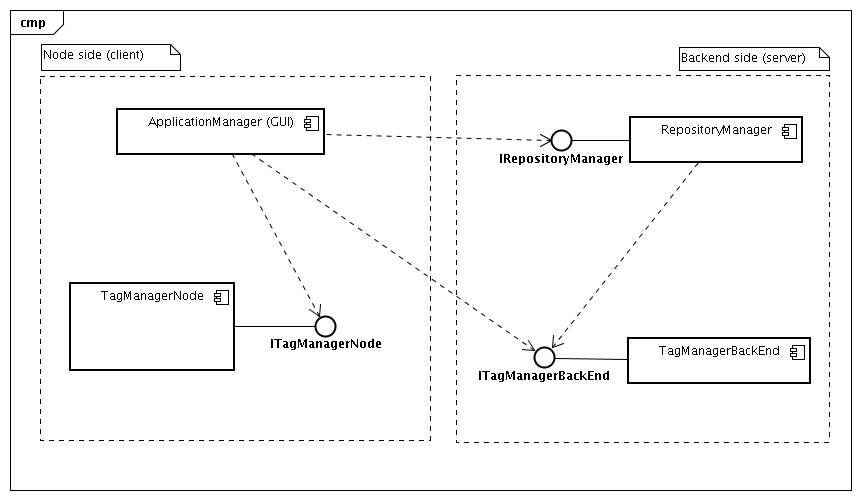
\includegraphics[scale=0.18]{img/BundlesComponentsDiagram.png}
			\end{figure}
	    
	    \end{column}
	
\end{columns}

\end{frame}

\subsection{RepositoryManager}

\begin{frame}

	\frametitle{RepositoryManager} 
	
	\begin{itemize}
		\item One of the key pieces:
		
		\begin{itemize}
		        \item Offer services to share applications.
		        \item Offer services to retrieve applications.
		        \item Offer services to search applications by criteria (description,
		        tags, type or any)
		        \item Offer services to search applications by similarity (with
		        respect to a local application).
		        \item Storage of shared applications.
		        \item Functionalities to adapt the application.
		        \item etc.
	    \end{itemize} 
		
		\item It is executed in the Backend.

	\end{itemize}

\end{frame}


\begin{frame}


\begin{columns}

	\begin{column}{6cm}
	Connection with other bundles:
	
	\begin{itemize}
	  \item \texttt{CommunityManager}: retrieve information about relationship
	  between users, communities \& applications. Ex.: assure visibility.
	  \item \texttt{TagManagerBackEnd}: analyze tags to create search engine index.
	  \item \texttt{EventsManager}: keep track of events in TMBE. Ex.: search
	  engine index updated dynamically.
	  \item \texttt{PersistencyManager}: store data in the DB.
	\end{itemize}
		
	
	\end{column}
	
		\begin{column}{7cm}
	    
			\begin{figure}
			 	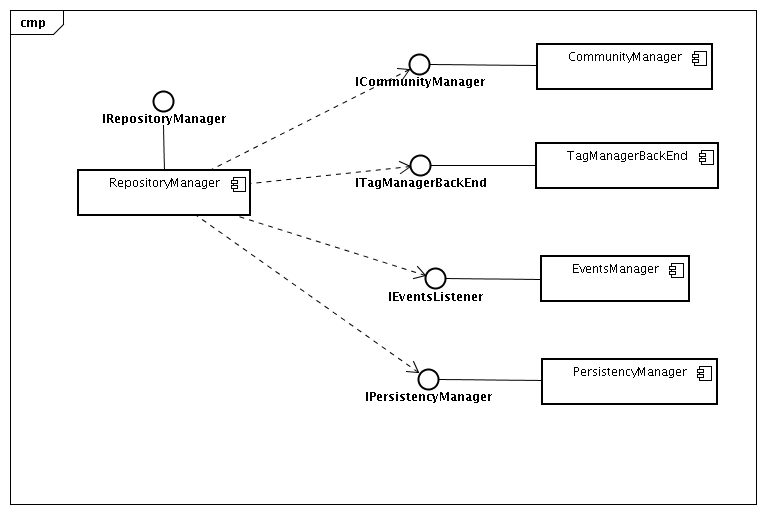
\includegraphics[scale=0.21]{img/RepositoryManagerComponentsDiagram.png}
			\end{figure}
	    
	    \end{column}
	
\end{columns}

\end{frame}


\begin{frame}
	    
	\begin{figure}
	 	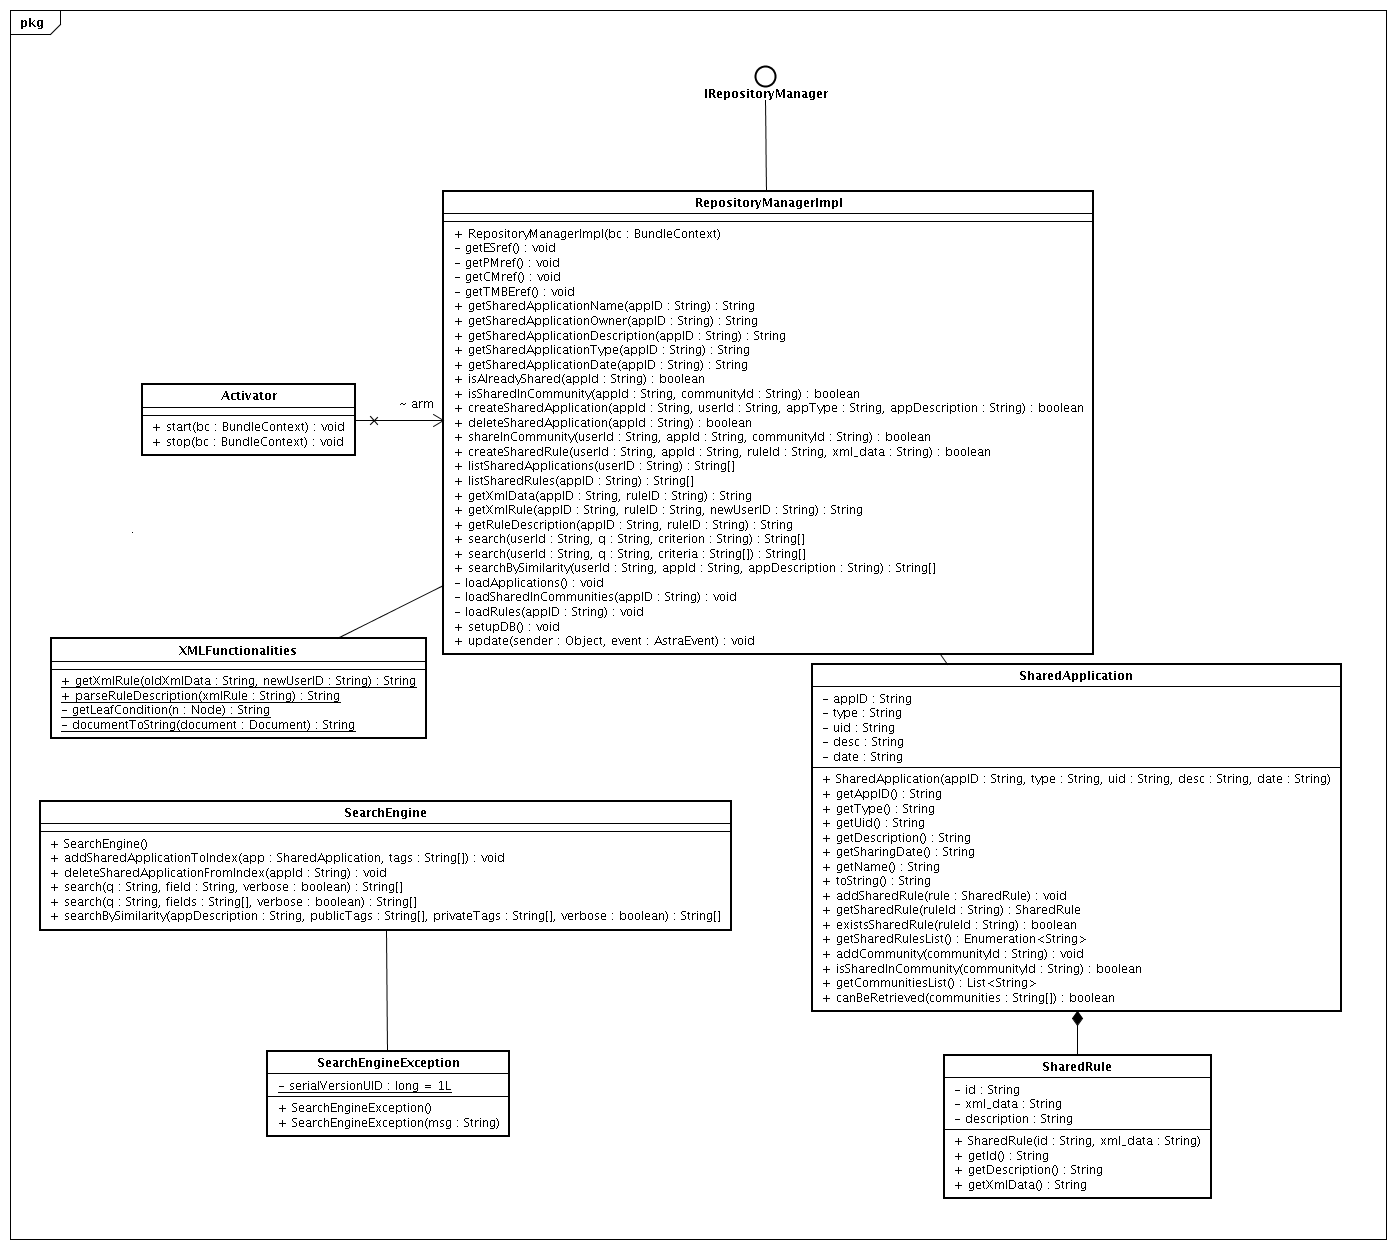
\includegraphics[scale=0.18]{img/RepositoryManagerClassDiagram.png}
	\end{figure}

\end{frame}


\begin{frame}
	
	Storage in DB:
	
	\begin{figure}
	 	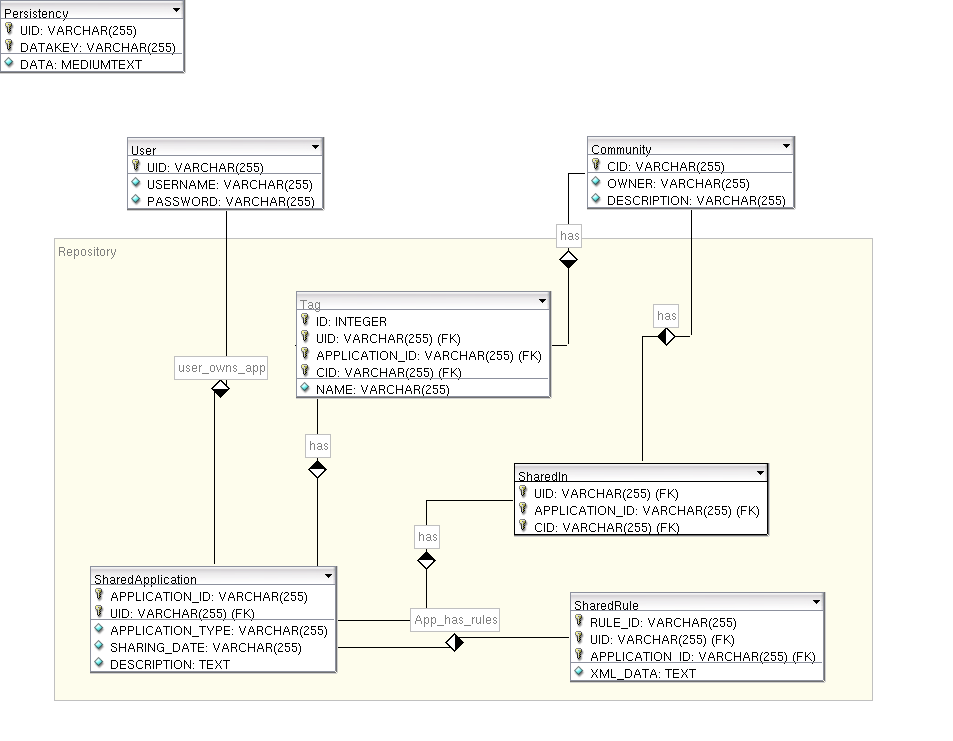
\includegraphics[scale=0.18]{img/RepositoryManagerDBModel.png}
	\end{figure}

	+ a synchronized copy in local memory to increase retrieving operations
	performance (drawback: duplicated create/delete operations).

\end{frame}




\subsection{TagManagerBackEnd}

\begin{frame}

\frametitle{TagManagerBackEnd}

	\begin{itemize}
		\item Offer services to add and delete public and community tags.
		\item Offer services to retrieve those tags in different and 
			flexible ways: by visibility, by communities, only public ones, etc.
		
	
		\item It is executed in the Backend.

	\end{itemize}

\end{frame}


\begin{frame}


\begin{columns}

	\begin{column}{6cm}
	Connection with other bundles:
	
	\begin{itemize}
	  \item \texttt{CommunityManager}: retrieve information about relationship
	  between users, communities \& tags. Ex.: assure visibility.
	  \item \texttt{EventsManager}: give feedback of the events.
	  \item \texttt{PersistencyManager}: store data in the DB.
	\end{itemize}
		
	
	\end{column}
	
		\begin{column}{7cm}
	    
			\begin{figure}
			 	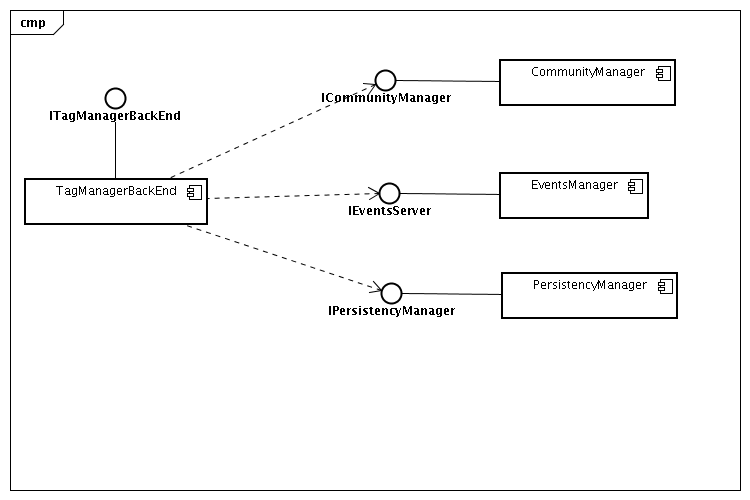
\includegraphics[scale=0.21]{img/TagManagerBackEndComponentsDiagram.png}
			\end{figure}
	    
	    \end{column}
	
\end{columns}

\end{frame}

\begin{frame}
	    
	\begin{figure}
	 	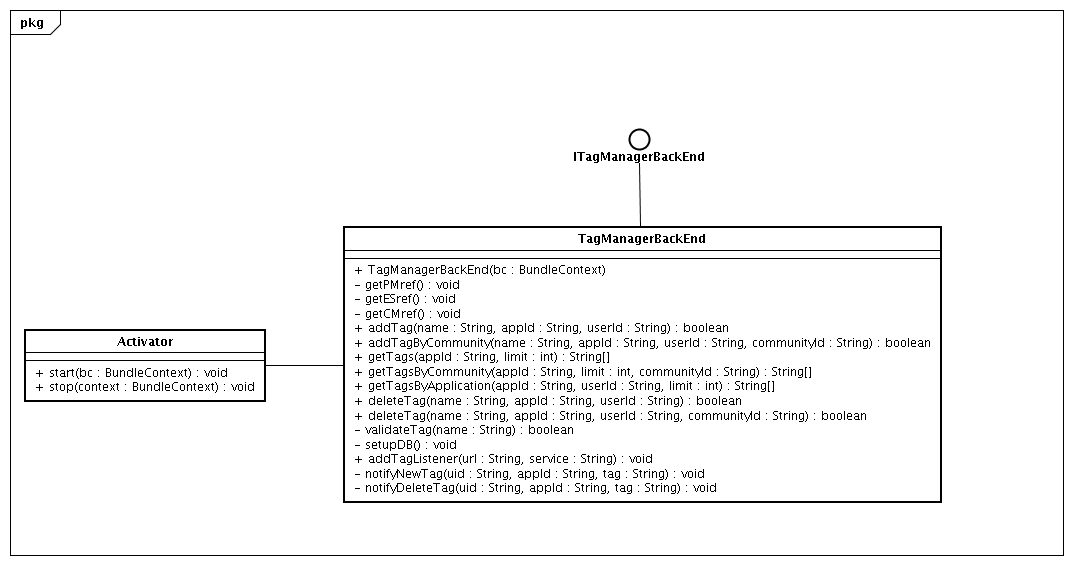
\includegraphics[scale=0.3]{img/TagManagerBackEndClassDiagram.png}
	\end{figure}

\end{frame}

\subsection{TagManagerNode}

\begin{frame}
\frametitle{TagManagerNode}

\begin{columns}

	\begin{column}{6cm}
	
	
	\begin{itemize}
		\item Offer services to add and delete private tags.
		\item Offer services to retrieve those tags in different and 
			flexible ways.
		\item It is executed in the Nodes.

	\end{itemize}
		
	
	\end{column}
	
		\begin{column}{7cm}
	    
			\begin{figure}
			 	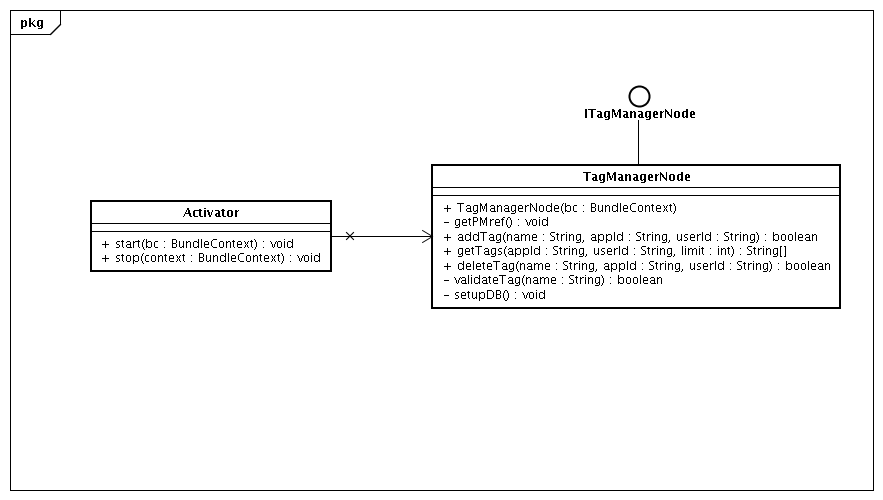
\includegraphics[scale=0.2]{img/TagManagerNodeClassDiagram.png}
			\end{figure}
	    
	    \end{column}
	
\end{columns}

\end{frame}

\subsection{ApplicationManager}

\begin{frame}
\frametitle{ApplicationManager}

	\begin{itemize}
		\item It is in charge of the interaction with the user by offering an
		intuitive GUI.
		\item Responsible of the connection with other ASTRA bundles services based
		on that interaction.	
		\item It is executed in the Nodes.
		\item It is connected with bundles from both edges: Node and Backend.
	\end{itemize}

\end{frame}

\begin{frame}
Connection with other bundles:

\begin{itemize}
  \item Local bundles:
	\begin{itemize}
	  \item \texttt{AwarenessApplicationManager}:  information about local applications.
	  \item \texttt{AwarenessManager}: information about local rules.
	  \item \texttt{TagManagerNode}: to manage the private tags.
	  \item \texttt{OntologyManager}: to assist the user in the application
	  adaptation process using ontologies\footnote{Future work.}.
    \end{itemize}
   
   \item Remote bundles:
	\begin{itemize}
	  \item \texttt{UserManager}: users authentication.
	  \item \texttt{CommunityManager}: information about the
	  communities joined by the user.
	  \item \texttt{TagManagerBackend}: to manage the public and community
	  tags.
	  \item \texttt{RepositoryManager}: to share and retrieve applications
	  with the rest of the users.
    \end{itemize}
    
\end{itemize}

\end{frame}


\begin{frame}
	    
	\begin{figure}
	 	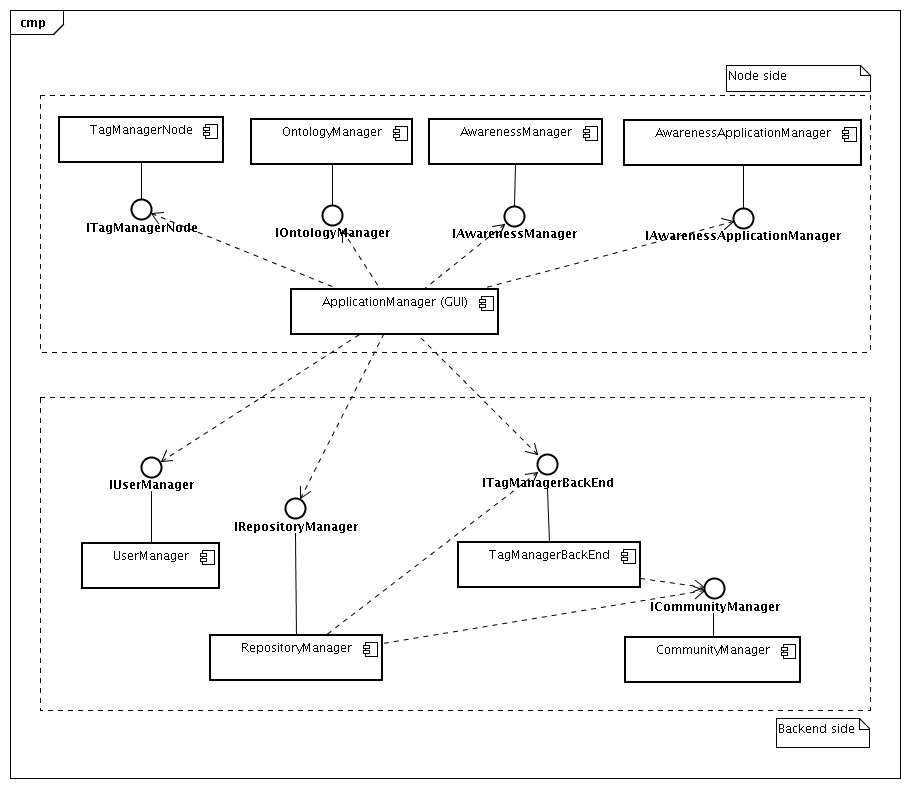
\includegraphics[scale=0.27]{img/ApplicationManagerComponentsDiagram.png}
	\end{figure}

\end{frame}

\begin{frame}

\begin{columns}

	\begin{column}{8cm}
	
	
	\begin{itemize}
		\item It implements a MVC (Model-View-Controller) pattern, which
			allows us to isolate the business logic from the user interface, permitting
			one to be freely modified without affecting the other.
		\item Some of the classes make use of a singleton pattern, that make the 
		class itself responsible for keeping track of its sole instance, ensuring 
		that no other instance can be created.
	\end{itemize}
		
	
	\end{column}
	
		\begin{column}{4cm}
	    
			\begin{figure}
			 	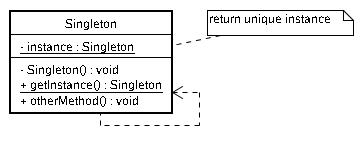
\includegraphics[scale=0.3]{img/singleton.jpg}
			\end{figure}
	    
	    \end{column}
	
\end{columns}

\end{frame}


\begin{frame}

\begin{itemize}
	\item Controller: 
	\begin{itemize}
        \item It is represented by the class
        \texttt{ApplicationManagerController} (singleton).
  		\item Keep track of references to user interface components.
  		\item Provide a set of methods that other components can directly call in
  		their event handler.
    \end{itemize}
    
 	\item Model:
		\begin{itemize}
	        \item It is represented by the class
	        \texttt{ApplicationManagerModel} (singleton).
	  		\item Manage the references to the rest of the bundles.
	  		\item Work as an ``stub container'' to make use of the services provided
	  		by those.
	  		\item Take care of the session data, i.e.: the user identifier.
	    \end{itemize}
    
    \item View: 
		\begin{itemize}
	        \item It is represented by several classes whose task consist of
    			presenting the information to the user.
	  		\item Includes all the classes which represent the windows (i.e.:
	  		\texttt{MainWindow}, \texttt{LoginWindow}, etc.) and all the classes that
	  		extend some of the graphical components (i.e.: \texttt{TreeRenderer}).
	  	\end{itemize} 
\end{itemize}

\end{frame}


% Skipped for time limit reasons
% \begin{frame}
% 
% 	\begin{figure}
% 	 	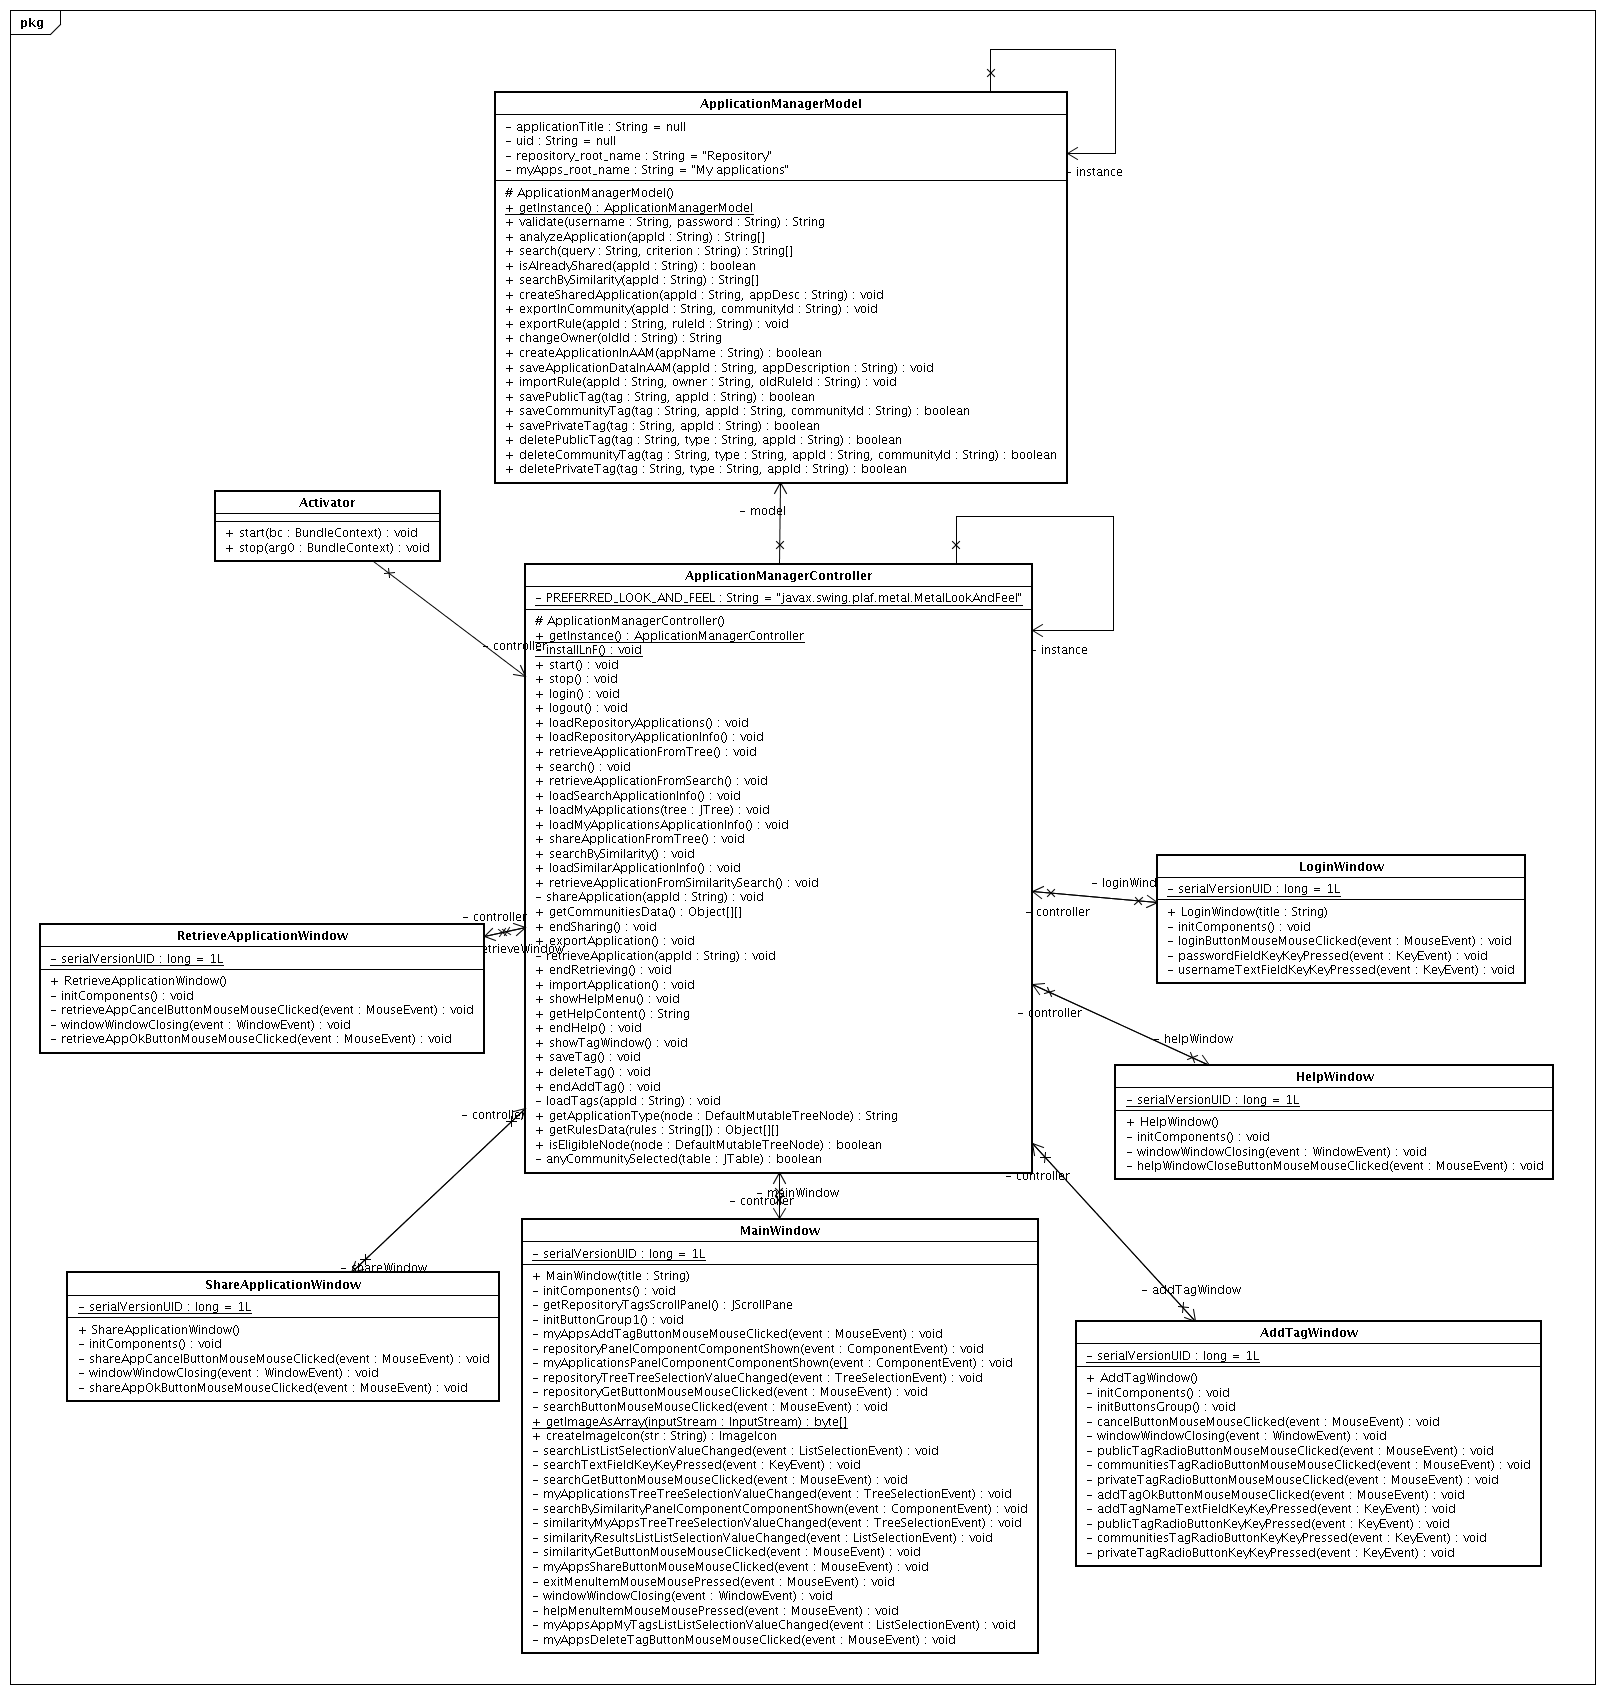
\includegraphics[scale=0.13]{img/ApplicationManagerClassDiagramSmall.png}
% 	\end{figure}
% 
% \end{frame}